% Este arquivo .tex será incluído no arquivo .tex principal. Não é preciso
% declarar nenhum cabeçalho

\section{Lugares para estudar}

Há vários lugares para estudar na Unicamp. Você pode escolher o que você achar
melhor:


\subsubsection{Biblioteca Central (BC):} A BC tem três andares. O primeiro é
onde tem os livros gerais e onde a galera estuda. Geralmente é barulhento em
épocas de provas, mas é bom porque sempre tem lugar para estudar e fecha às 22h.
Se você não se importa com barulho, ou até acha que você faz bastante, esse é o
lugar da BC para você estudar. O segundo andar é onde está a BAE, a Biblioteca
da Área de Engenharia. Um pouco mais silenciosa que a BC nas mesas externas,
esse andar tem salas para estudo em grupo, bastante silenciosas, mas que sempre
estão ocupadas em época de provas, e mesas individuais escondidas entre os
periódicos. O terceiro andar é para silence freaks. Morbidamente silencioso,
desértico (muita gente desconhece a existência desse andar), esse é o lugar mais
silencioso da BC para estudar. Tem umas salinhas de estudo individual e duas
mesas para estudo em grupo. O problema é que fecha às 17h, mas o pôr-do-sol de
lá de cima também é ma-ra-vi-lho-so.

\begin{figure}[h!]  \centering
  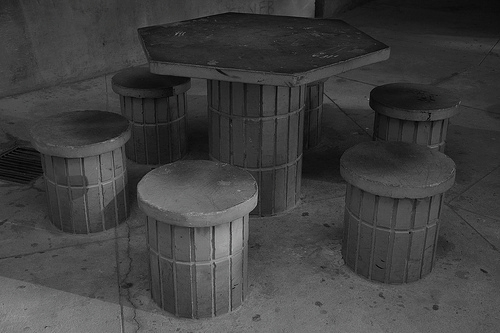
\includegraphics[width=.45\textwidth]{img/unicamp/mesinhas.jpg}
\end{figure}

\subsubsection{Arcádia (ou mesinhas do IEL):} A Arcádia é algumas mesas ao ar
livre no IEL (Instituto de Estudos da Linguagem). Em horários de aula é
silencioso, é um ambiente muito agradável e por ser ao ar livre, não fecha.  Tem
dois problemas: O grande fluxo de pessoas no local pode facilmente distraí-lo,
principalmente se você as conhecer, e à noite enche de insetos (além da
iluminação não ser das melhores). Às vezes, venta bastante e é ruim para estudar
com folhas avulsas. Mas ainda assim é um ótimo local para estudar.

\subsubsection{Biblioteca do IFGW:} A biblioteca do IFGW (Instituto de Física
Gleb Wataghin) é ótima para dias de calor, por ser super gelada (ar-condicionado
mega-super-power!). Tem vantagem sobre as outras bibliotecas pelo fato das salas
de estudo serem fora da biblioteca e por isso você não precisa deixar o seu
material para entrar na sala de estudos. Recentemente reformada, agora conta com
6 salas para estudo em grupo e quantidade razoável de baias individuais, algumas
com tomadas onde você pode plugar seu notebook. As salas em grupo passaram a
ficar trancadas, é preciso deixar o RA pra pegar a chave, e algumas são
reservadas para alun*s da Física.

\subsubsection{BIMECC:} A biblioteca do IMECC tem poucos lugares, poucas mesas
para estudo individual, os locais de estudo ficam dentro da biblioteca (você
precisa guardar sua bolsa para entrar), não é muito gelada e o ambiente não é
agradável, mas nela e na BAE é que você encontrará a maioria dos livros
relacionados a computação.

\subsubsection{Outras bibliotecas:} Aventure-se por outras bibliotecas, como a
da Economia, a da Pedago e a da Biologia e as conheça. Para aqueles que gostam
(ou são obrigados) a estudar aos fins de semana a BC e as bibliotecas da
Educação, da Economia, da Química, da Medicina, do IEL e da Geociências abrem
aos sábados. Para saber os horários de funcionamento das bibliotecas, entre no
site do SBU (\url{www.sbu.unicamp.br/portal/index.php?Itemid=139}).

\subsubsection{Bitolódromos:} Existem dois bitolódromos na Unicamp: O do IC e o
da FEEC (coincidência interessante, né?). O do IC-3 é uma mesa grande com
algumas cadeiras no corredor dos laboratórios. O da FEEC fica no fundo do prédio
principal (qualquer veteran* sabe onde é o bitolódromo, não tenha vergonha de
perguntar). O da FEEC é maior, você se distrai menos porque não estão todos os
seus colegas (mas várias outras pessoas estão) entrando e saindo de lá (embora
*s pica-fios sejam bastante barulhentos), e sempre você encontra gente que possa
te ajudar.  O do IC serve para quando você já estiver lá e com preguiça de ir à
Elétrica, porque o da FEEC é muito melhor. Recentemente abriram um novo
bitolódromo na FEEC, no fim do corredor que leva ao SIFEEC, mas tudo indica que
esse espaço é temporário, talvez ele não exista mais no momento em que você está
lendo isso.

\subsubsection{Sala 316:} Outro alento para as madrugadas de estudo é a sala 316
do IC-3, que fica aberta sempre, ou então, aberta facilmente com a chave em
posse d* guardinha. É uma sala com carteiras legais, lousa e ar condicionado,
aliás, é muito boa para estudo em grupo (NABVS IMINENTVS) por causa da lousa.

\begin{figure}[h!]  \centering
  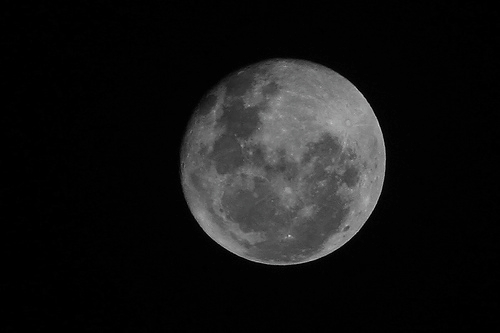
\includegraphics[width=.45\textwidth]{img/unicamp/lua.jpg}
\end{figure}

\subsubsection{Sua casa:} Se você mora em uma república com pessoas da sua
turma, vá fundo e estude em casa. Se você mora sozinh* ou com pessoas de outros
cursos/anos, mas se concentra bem em casa, também o faça. Caso contrário, estude
na Unicamp. É muito fácil se distrair em casa. Você vai à geladeira, mexe no
computador, lê outra coisa, deita na cama e dorme, entre outras coisas. Prefira
estudar na Unicamp. Outra coisa, não seja egoísta, quando tiver oportunidade de
estudar em grupo, prefira essa alternativa. Lembre-se que você não está mais no
``cursinho'', tente sempre pegar as dicas que a galera te dá, principalmente d*s
seus(suas) veteran*s.

